\documentclass{ikpKoeln}
\usepackage{graphicx}
\usepackage{physics}
\usepackage{xcolor}
\usepackage{tikz}
\usetikzlibrary{math}

\scTitle{Experimenting on a new method for the NeuLAND position calibration and fine tuning with the Millepede algorithm}
\scAuthor{*}{Yanzhao}{Wang}{1}
\scAuthor{}{Igor}{Gasparic}{2}
\scAuthor{}{Håkan}{Johansson}{3}
\scAuthor{}{Andreas}{Zilges}{1}
\scAffiliation{1}{University of Cologne, Institute for Nuclear Physics, Germany}
\scAffiliation{2}{GSI Helmholtzzentrum für Schwerionenforschung, Germany}
\scAffiliation{3}{Chalmers University of Technology, Sweden}

\scTitleShort{Millepede algorithm for the position calibration of NeuLAND}

\date{\scriptsize R3B Collaboration Meeting \\ July 8th 2024}

\graphicspath{{../figures/}}

\addbibresource{reference.bib}

\begin{document}

\begin{frame}[t]{Time and position calibration parameters}
	\vspace{-1cm}
	\begin{columns}[t]
		\begin{column}{0.4 \textwidth}
			\vspace*{-0.5cm}
			\begin{figure}[t]
				\hspace*{-0.5cm}
				\centering
				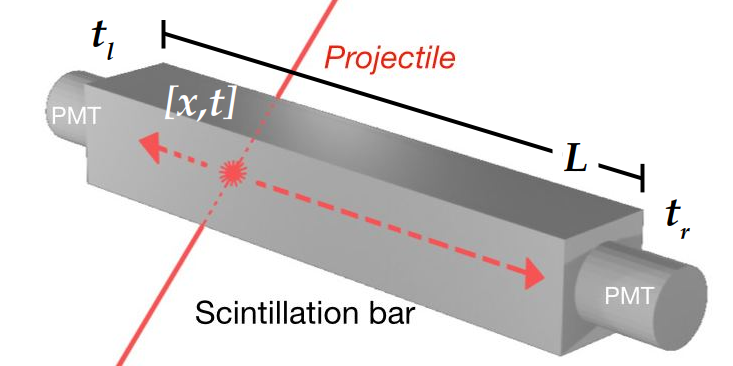
\includegraphics[keepaspectratio, height = 0.4\textheight]{R3BCon2024GSI/Bar.png}
			\end{figure}
			\vspace{0.5cm}
			\textit{Symbols}:
			\scriptsize{
				\begin{flalign*}
					x           & : \text{position of the interaction } & \\
					t           & : \text{time of the interaction}      & \\
					L           & : \text{length of the scintillator}   & \\
					t_l         & : \text{time of the left PMT signal}  & \\
					t_r         & : \text{time of the right PMT signal} & \\
					\alert{C_e} & : \text{effective speed of light}     & \\
				\end{flalign*}
			}
		\end{column}
		\begin{column}{0.48 \textwidth}
			\begin{block}{\small Time relation:}
				$$ t = \frac{t_r + t_l}{2} - \frac{L}{2 \cdot \alert{C_e}} + \alert{t_\text{sync}}$$
			\end{block}

			\begin{block}{\small Position relation:}
				$$ x = \frac{\alert{C_e}}{2}\left( t_r - t_l  + \alert{t_\text{offset}} \right)$$
			\end{block}

			{ \small
			\textit{Additional calibration parameters:}
			\begin{itemize}
				\item \alert{$t_\text{sync}$} : time synchronization among scintillators \\
				\item \alert{$t_\text{offset}$} : time offset between adjacent PMTs
			\end{itemize}
			}

			\vspace{0.5em}
			\textit{Total number of calibration parameters: \alert{\Large{3900}}}
		\end{column}
	\end{columns}
\end{frame}

\begin{frame}[t]{Current calibration method}
	\vspace*{-2em}
	\begin{columns}[t]
		\begin{column}{0.45 \textwidth}
			\begin{figure}[t]
				\includegraphics<1>[width = \textwidth]{R3BCon2024GSI/side_view1.png}
				\includegraphics<2>[width = \textwidth]{R3BCon2024GSI/side_view2.png}
				\includegraphics<3-5>[width = \textwidth]{R3BCon2024GSI/side_view3.png}
				\includegraphics<6>[width = \textwidth]{R3BCon2024GSI/side_view4.png}
			\end{figure}
		\end{column}
		\begin{column}{0.45 \textwidth}
			\begin{exampleblock}{\small Procedures}
				\small
				\begin{enumerate}
					\setlength\itemsep{0em}
					\small
					\item<1-> Obtain the positions of bars with signals
					\item<2-> Reconstruct the muon track from the bar positions
					\item<3-> Calculate the positions of the interaction points of the muon
					\item<4-> Calculate the calibration parameters via data fitting
				\end{enumerate}
			\end{exampleblock}
			\onslide<5->{
				\vspace*{-0.5em}

				\textit{\small Data fitting in the position calibration:}\par
				\vspace*{-0.5em}

				\begin{figure}[t]
					\centering
					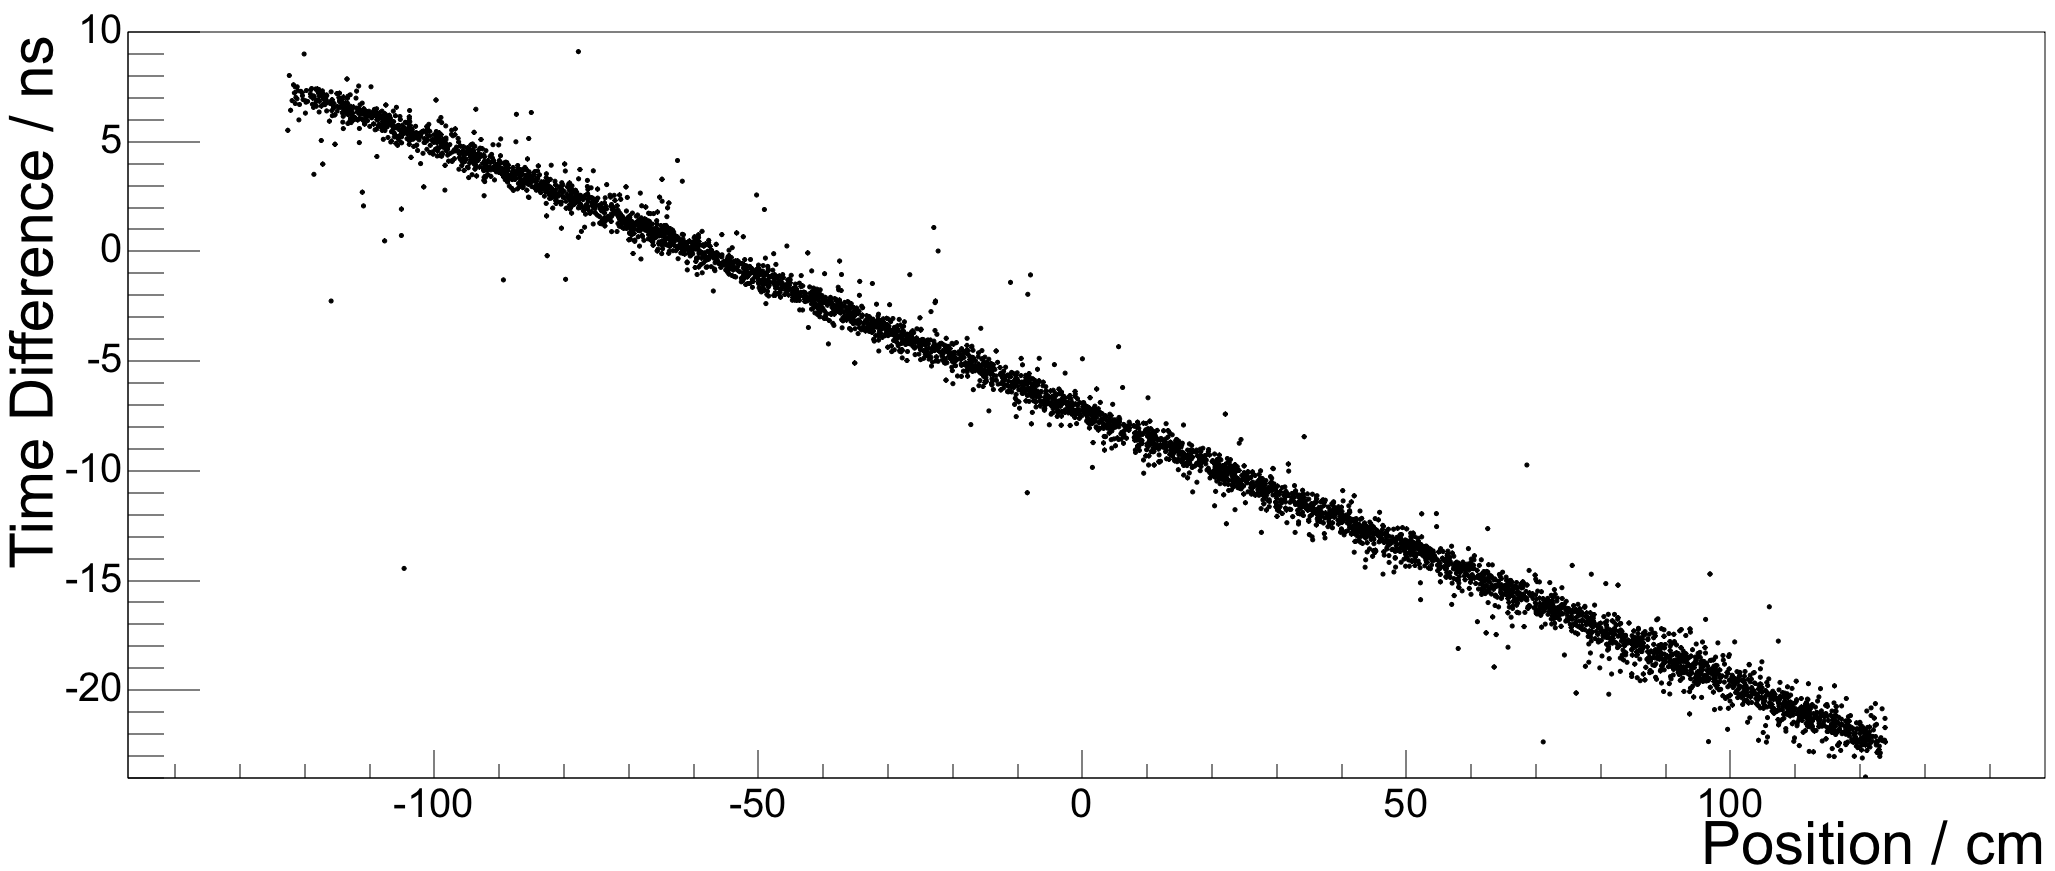
\includegraphics[ width = \textwidth]{R3BCon2024GSI/time_cal.png}
				\end{figure}
			}
		\end{column}
	\end{columns}
\end{frame}

\begin{frame}[t]{Simultaneous fitting using the Millepede algorithm}
	\begin{columns}[t]
		\begin{column}{0.48 \textwidth}
			\pause
			Calibration with muon tracks:
			\vspace*{-0.5em}
			\begin{align}
				\small
				\text{pos}  & = \alert{C_e}\cdot \left( t_r - t_l  + \alert{t_\text{offset}} \right) / 2            \\
				t           & = \slfrac{(t_r + t_l)}{2} - \slfrac{L}{(2 \cdot \alert{C_e})} + \alert{t_\text{sync}} \\
				\vec{x}_\mu & = \textcolor{blue}{\vec{a}^{\,i}} \cdot z_\mu  + \textcolor{blue}{\vec{b}^{\,i}}
			\end{align}
			\vspace*{-2em}

			{\scriptsize where $\vec{a} = (a_x, a_y, a_t)$, $\vec{b} = (b_x, b_y, b_t)$}\\

			\pause
			\vspace*{0.5em}
			{\footnotesize
			{\textit{For time offsets of horizontal bars:}}
			\vspace*{-0.5em}
			$$\textcolor{blue}{b^i_x} - \alert{g^i_{ct}} /2 + \alert{g^i_c} \cdot \Delta t^i / 2 + \textcolor{blue}{a^i_x} z_\mu         = 0 $$
			\textit{For time offsets of vertical bars:}
			$$\textcolor{blue}{b^i_y} - \alert{g^i_{ct}} /2 + \alert{g^i_c} \cdot \Delta t^i / 2+ \textcolor{blue}{a^i_y} \cdot z_\mu = 0 $$
			\textit{For time sync:}
			$$\textcolor{blue}{b^i_t}  + \alert{g^i_s} + L / (2 \cdot \alert{g^i_c}) - t_\text{sum} / 2 + \textcolor{blue}{a^i_t} z_\mu  = 0 $$
			\vspace{-2em}
			with $\alert{g^i_{c}} = \alert{C_e}$, $\alert{g^i_{ct}} = \alert{C_e} \cdot \alert{t_\text{offset}}$ and $\alert{g^i_s} = \alert{t_\text{sync}}$
			}
		\end{column}

		\begin{column}{0.48 \textwidth}
			\pause
			\textbf{Millepede input:}
			\vspace*{-0.5em}
			\begin{flalign*}
				\partial f/{\partial q_j} & : \text{1st order derivative of \textcolor{blue}{local parameters}} \\
				\partial f/{\partial p_l} & : \text{1st order derivative of \alert{global parameters}}          \\
				z                         & : \text{"measurements" (\textbf{constant values})}                  \\
				\sigma                    & : \text{measurement errors}
			\end{flalign*}

			\pause
			\vspace*{-1em}
			\begin{alertblock}{Solutions to the rank deficit error}
				\begin{itemize}
					\setlength\itemsep{0em}
					\item Reduce global or local parameters
					\item Applying additional constraints
				\end{itemize}
			\end{alertblock}
			\textit{Introducing local constraints:}
			\begin{flalign*}
				 & \text{Horizontal bars}: & \textcolor{blue}{b^i_y} - Y^i_{bar} + \textcolor{blue}{a^i_y} \cdot z_\mu = 0 \\
				 & \text{Vertical bars}:   & \textcolor{blue}{b^i_x} - X^i_{bar} + \textcolor{blue}{a^i_x} \cdot z_\mu = 0
			\end{flalign*}
		\end{column}
	\end{columns}
\end{frame}

\begin{frame}[t]{Predetermination of position parameters}
	\vspace*{-0.5em}
	\begin{exampleblock}{Purposes of predetermination}
		\begin{itemize}
			\item Use good initial values from a crude calibration method to reduce rejected entries ($< 33.3\%$)
			\item Select one bar from the plane when a muon crosses multiple bars of the same plane
			\item Remove outliners caused by background $\gamma$ rays
		\end{itemize}
	\end{exampleblock}
	\textbf{\footnotesize Step 1: Collect time differences of adjacent PMT signals}
	\vspace*{-1.8em}
	\begin{columns}[t]
		\begin{column}[t]{0.48\textwidth}
			\begin{figure}[t]
				\vspace*{-1em}
				\centering
				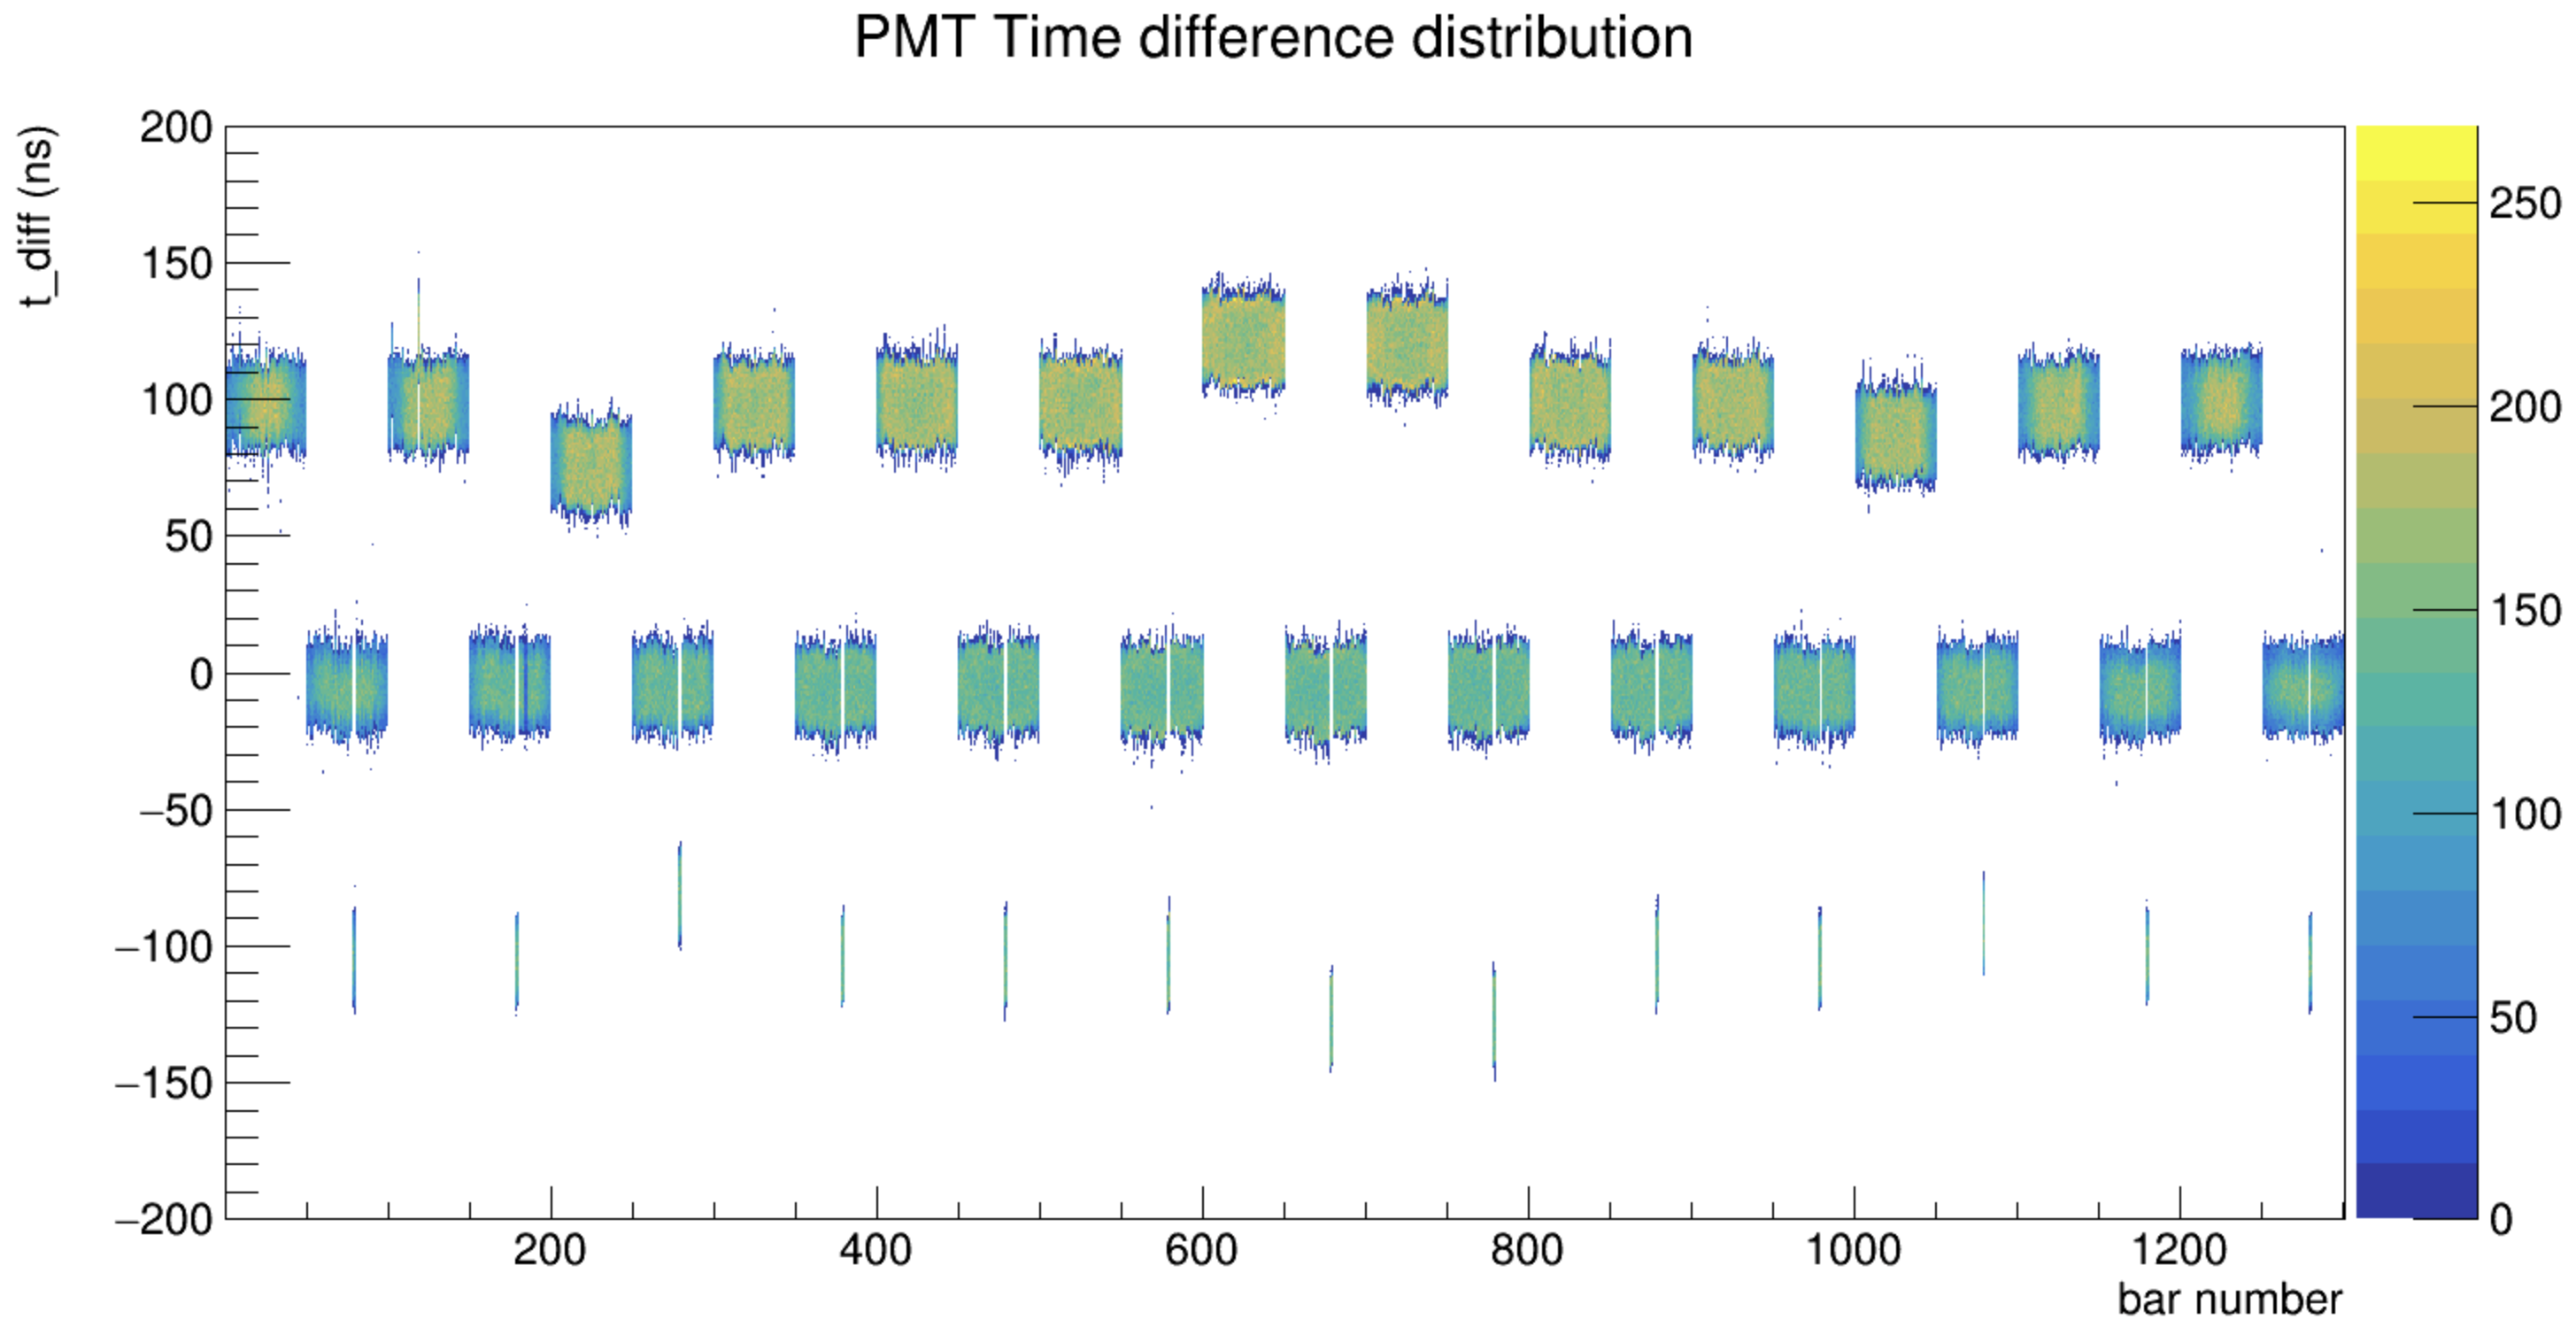
\includegraphics[height = 0.47\textheight]{R3BCon2024GSI/total_tdiff.png}
			\end{figure}
		\end{column}
		\begin{column}[t]{0.48\textwidth}
			\begin{figure}[t]
				\centering
				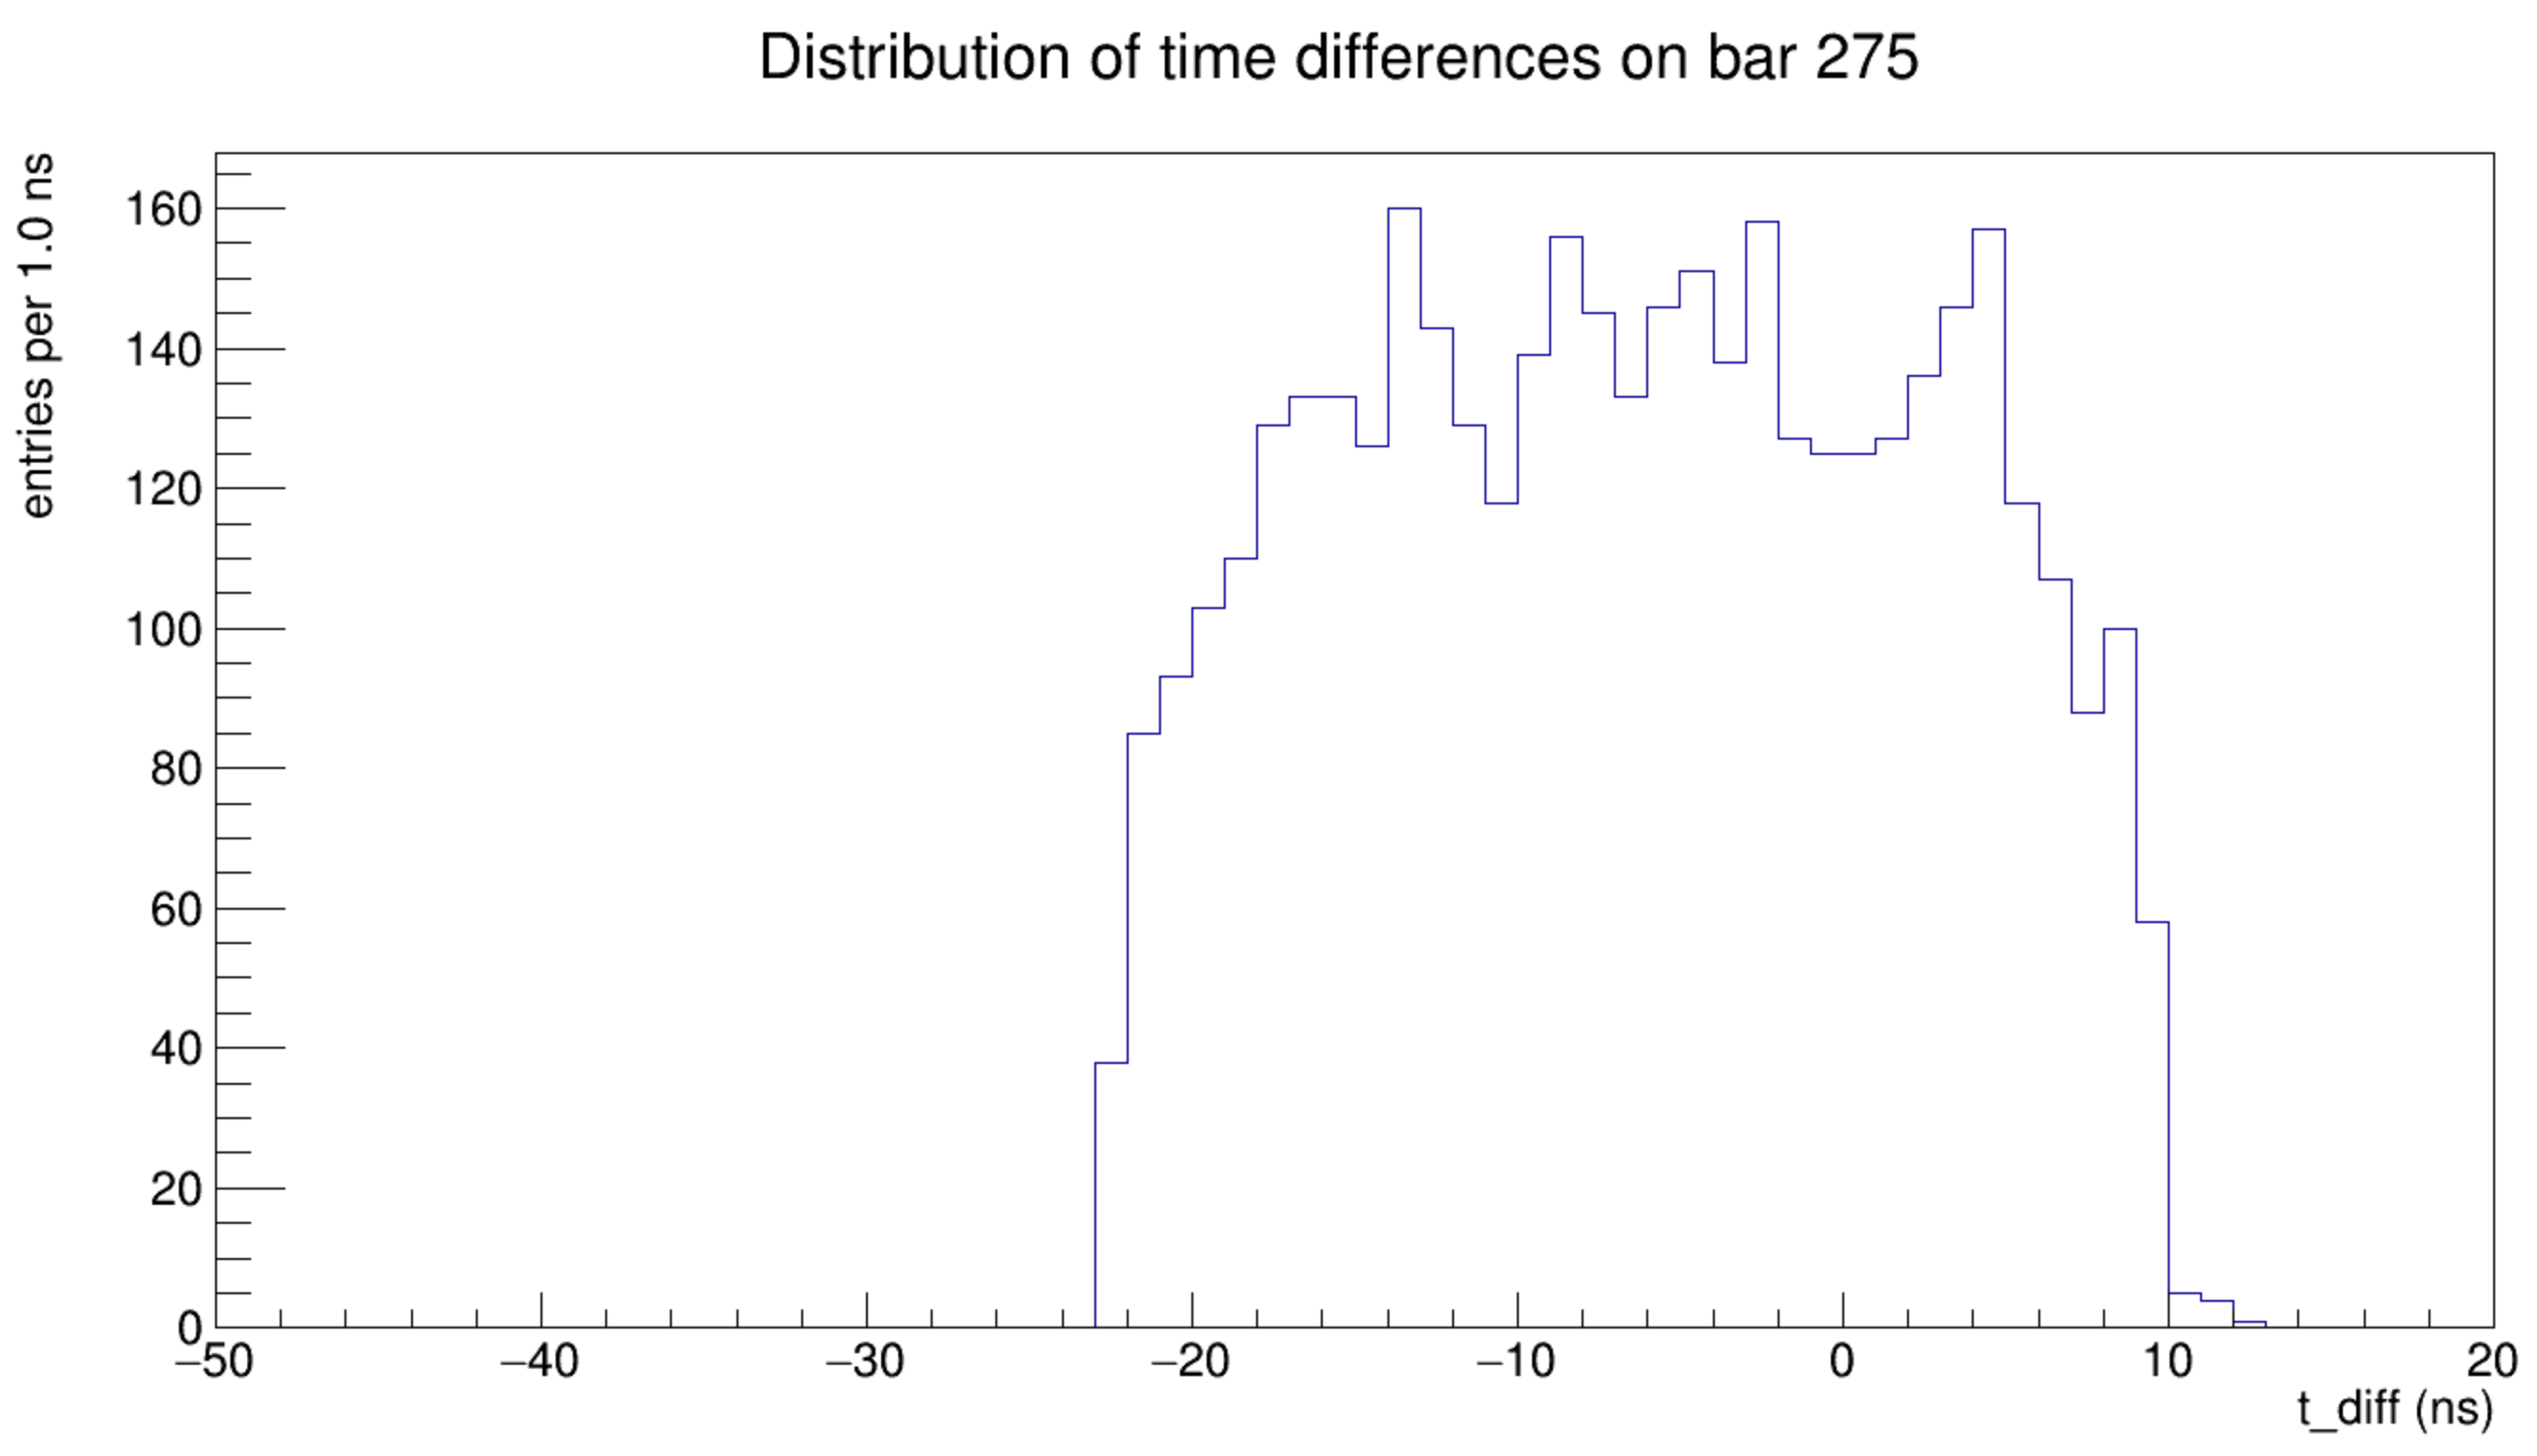
\includegraphics[height = 0.48\textheight]{R3BCon2024GSI/one_bar_tdiff.png}
			\end{figure}
		\end{column}
	\end{columns}
\end{frame}

\begin{frame}[t]{Predetermination on position parameters}
	\vspace*{-1em}
	\begin{columns}[t]
		\begin{column}[t]{0.48\textwidth}
			\textbf{\footnotesize Step 2: Normalize the distribution and convert to a CDF for each bar}\\
			\begin{figure}[t]
				\vspace*{-0.5em}
				\centering
				\includegraphics<1>[height = 0.47\textheight]{R3BCon2024GSI/CDF_275.png}
				\includegraphics<2->[height = 0.47\textheight]{R3BCon2024GSI/CDF_275_fitted.png}
			\end{figure}
			\onslide<2->{
				\footnotesize
				\vspace*{-1.5em}
				\textbf{Step 3: Linear fitting from 0.05 to 0.95}\\
				\begin{exampleblock}{\scriptsize Calculation of parameters:}
					\vspace*{-1.5em}
					\begin{align*}
						C_e               & = 2 \cdot \text{BarLength} \cdot \text{slope} \\
						t_{\text{offset}} & = (0.5 - \text{intercept}) / \text{slope}
					\end{align*}
				\end{exampleblock}
			}
		\end{column}
		\begin{column}[t]{0.48\textwidth}
			\onslide<3->{
				\textbf{\footnotesize Evaluation results:}\\
				\begin{figure}[t]
					\vspace*{-0.5em}
					\centering
					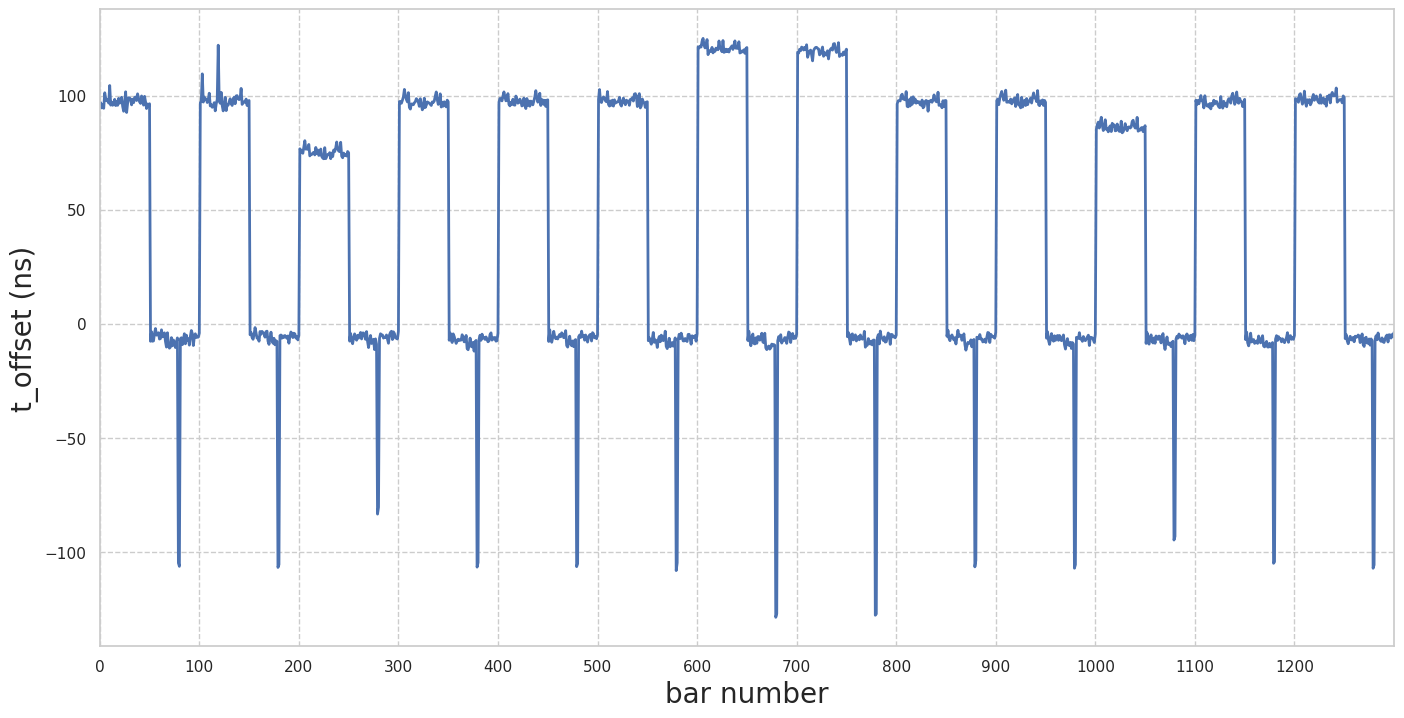
\includegraphics[width = 0.95\textwidth]{R3BCon2024GSI/t_offset_pre.png}
					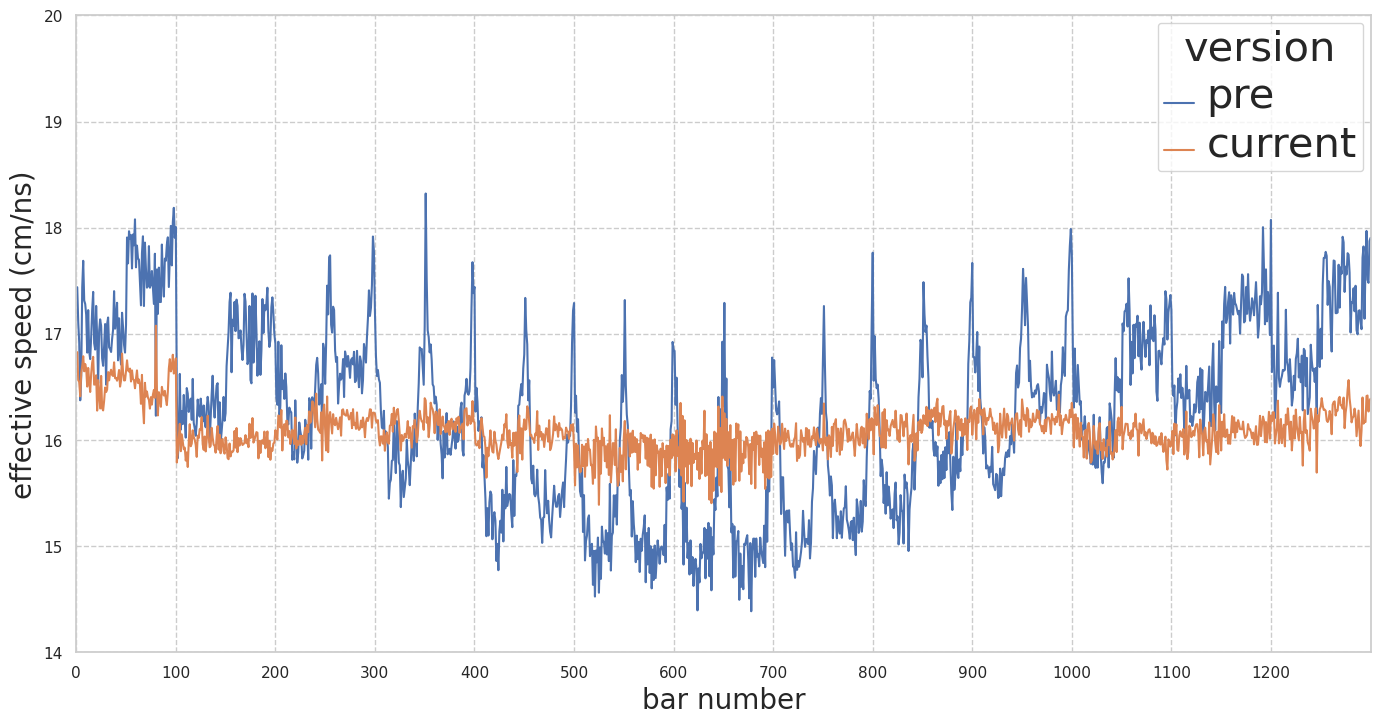
\includegraphics[width = 0.95\textwidth]{R3BCon2024GSI/effective_c.png}
				\end{figure}
			}
		\end{column}
	\end{columns}
\end{frame}

\begin{frame}[t]{Fine tuning with the Millepede algorithm}
	\vspace*{-1.2em}
	\begin{columns}[t]
		\begin{column}[t]{0.48 \textwidth}
			\begin{block}{Data preprocessing}
				\begin{enumerate}
					\item Scale the time/position values ($\times 10^{-1}$)
					\item Select bars with only one signal per event
					\item Remove the isolated bars of each plane
					\item Average bar positions for local constraints
					\item Linear fit with $z-x$ and $z-y$ functions on bar positions
					\item Choose the bar closest to the linear function for each plane
					\item Remove bars with large residuals
				\end{enumerate}
			\end{block}
		\end{column}
		\begin{column}[t]{0.48 \textwidth}
			\vspace*{-1em}
			\begin{figure}[t]
				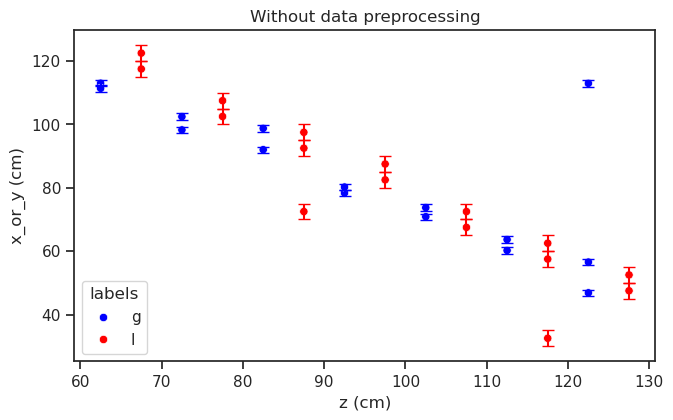
\includegraphics[width = 0.8\textwidth]{R3BCon2024GSI/local_unfit.png}
				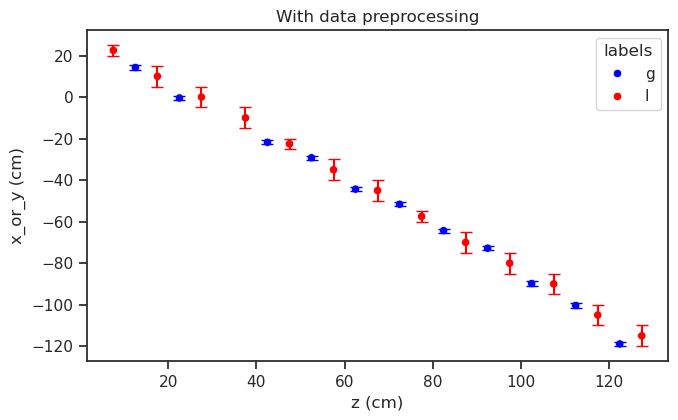
\includegraphics[width = 0.8\textwidth]{R3BCon2024GSI/local_fit.png}
			\end{figure}
		\end{column}
	\end{columns}
\end{frame}

\begin{frame}{Comparison of time offset parameters}
	\begin{figure}[t]
		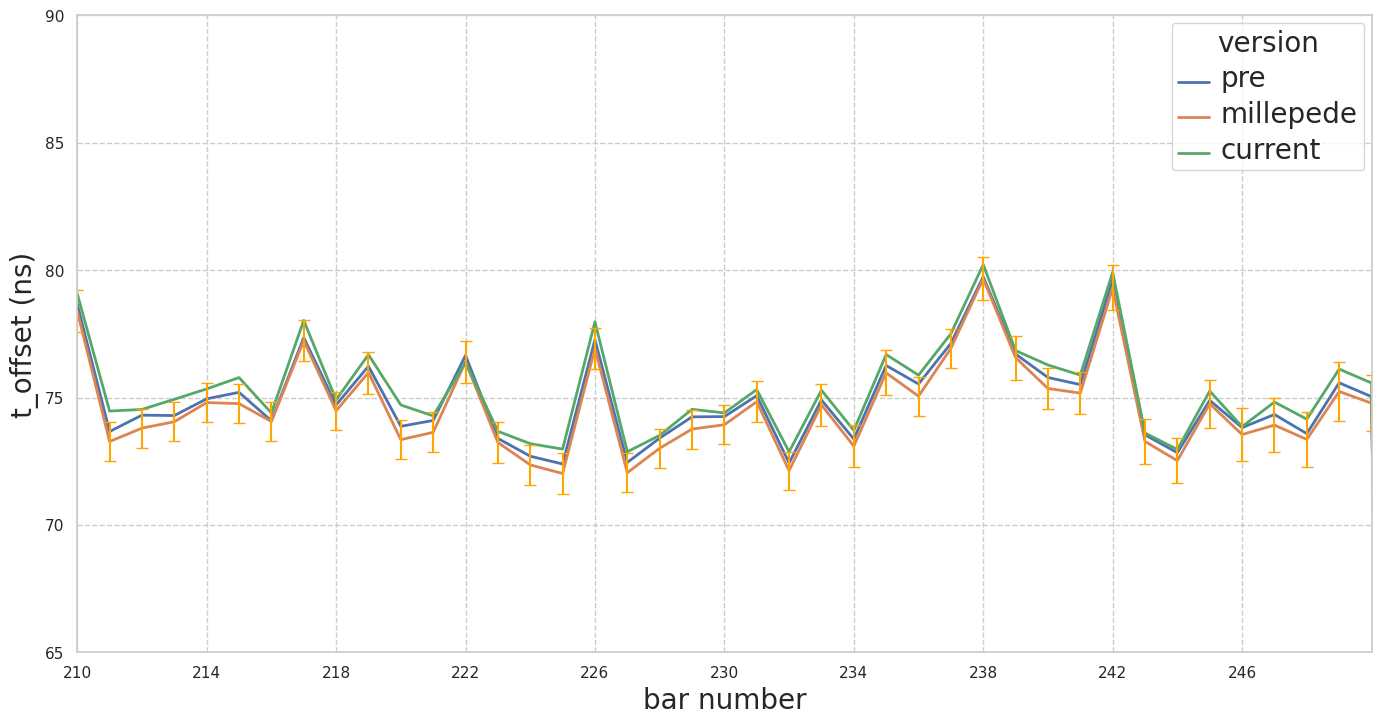
\includegraphics[width = 0.95\textwidth]{R3BCon2024GSI/toffset_comp.png}
	\end{figure}
\end{frame}

\begin{frame}{Comparison of effective speed parameters}
	\begin{figure}[t]
		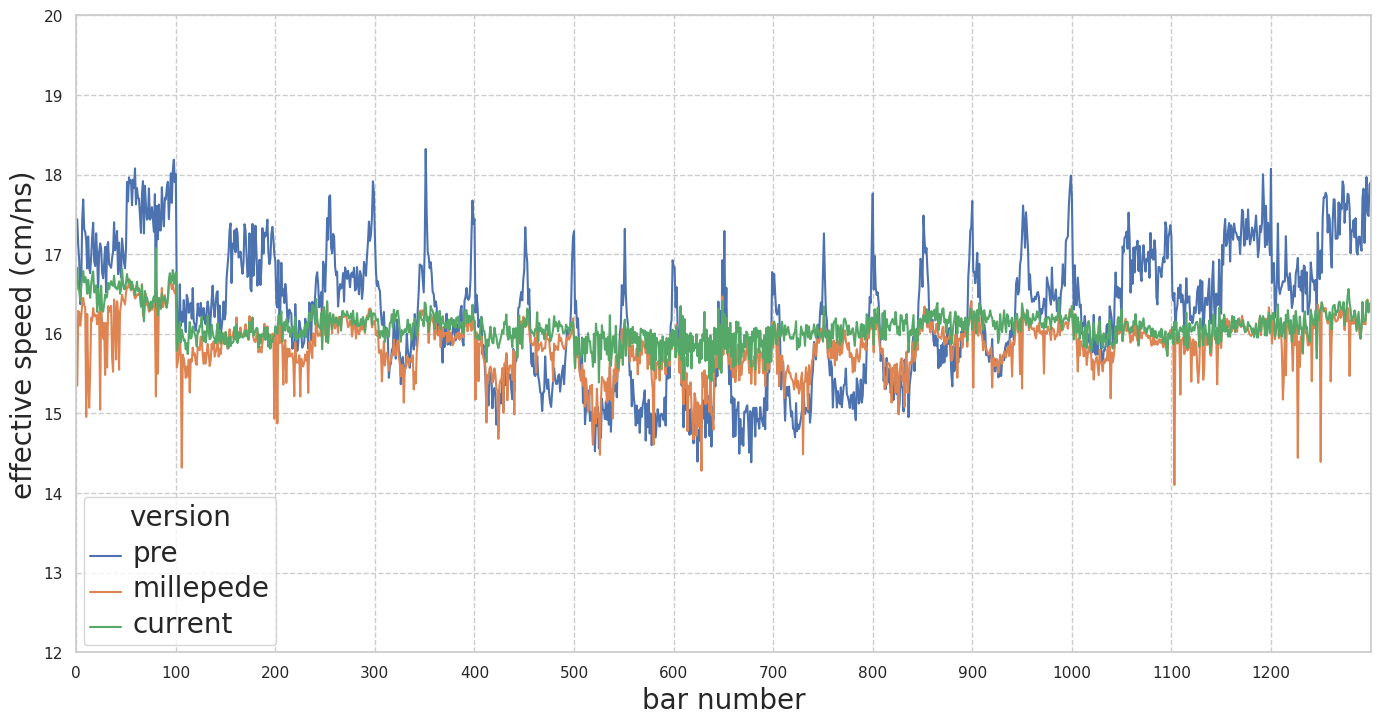
\includegraphics[width = 0.95\textwidth]{R3BCon2024GSI/effective_c_comp.png}
	\end{figure}
\end{frame}

\begin{frame}{Summary and outlook}
	\footnotesize
	\begin{columns}
		\begin{column}{0.49\textwidth}
			\begin{block}{Summary}
				\begin{itemize}
					\item Simultaneous fitting using the Millepede algorithm
					\item Predetermination of the position-related calibration parameters
					\item Good consistency between the results from the Millepede algorithm and the current method
				\end{itemize}
			\end{block}
			\begin{exampleblock}{Outlook}
				\begin{itemize}
					\item Adding time synchronization parameters
					\item Applying the Millepede algorithm to the energy calibration
					\item Further comparison between the Millepede algorithm and current method with the simulated data
				\end{itemize}
			\end{exampleblock}
		\end{column}
		\begin{column}{0.49\textwidth}
			\begin{figure}[t]
				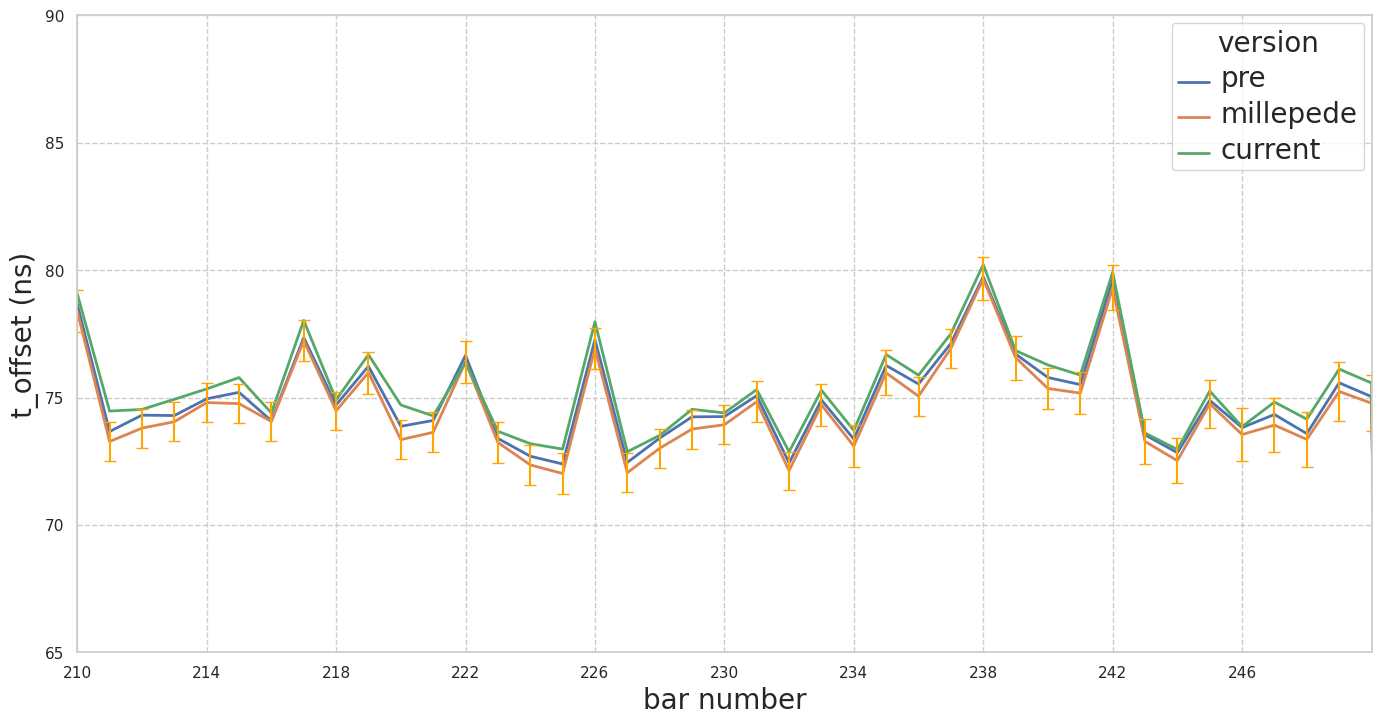
\includegraphics[width = 0.95\textwidth]{R3BCon2024GSI/toffset_comp.png}
				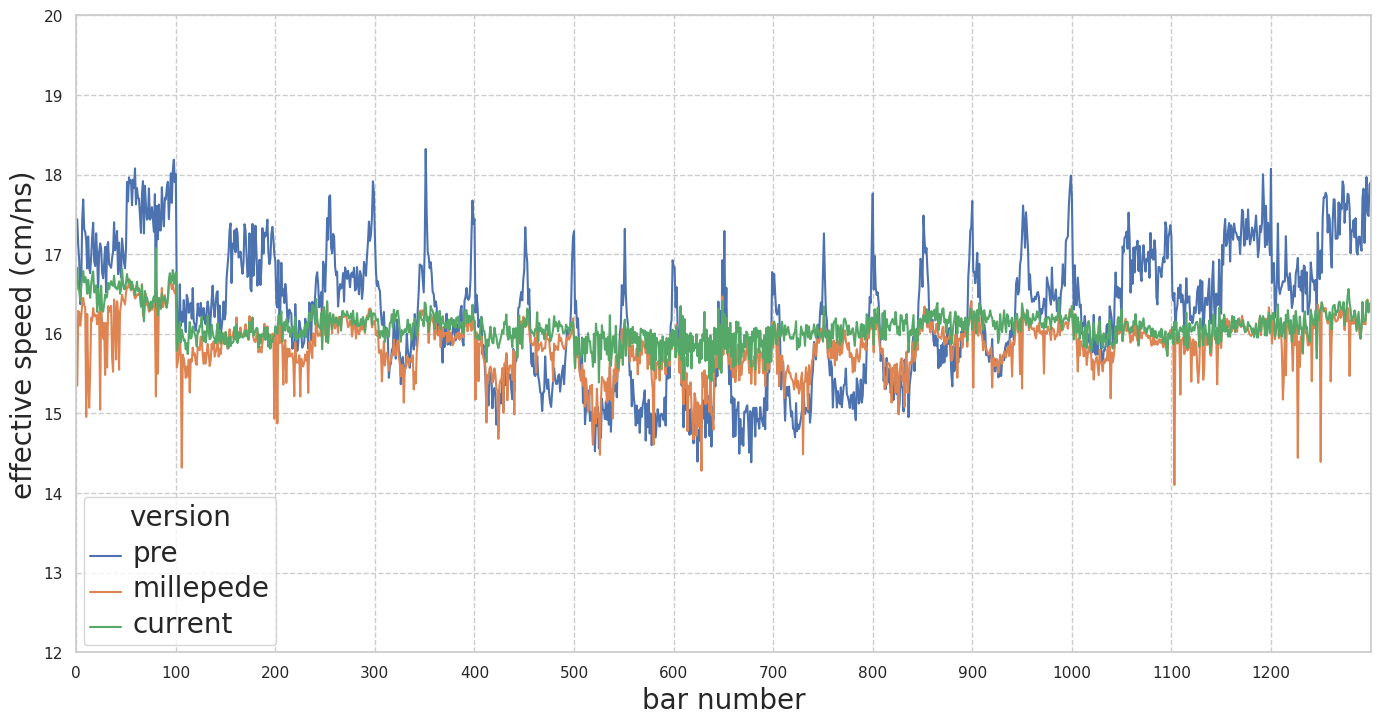
\includegraphics[width = 0.95\textwidth]{R3BCon2024GSI/effective_c_comp.png}
			\end{figure}
		\end{column}
	\end{columns}
\end{frame}

\end{document}
